\section{Comparison to other CPAs}
\subsection{Value analysis CPA}
Comparison to the \valueAnalysisCPA\ shows the strengths and weaknesses of symbolic execution, persisting even when using CEGAR:
Due to its higher precision, its computation is more reliable in comparison to the more abstract value analysis, finding 200~less non-existent errors.
But die to its higher precision, it also exceeds the time limit 535~times more often.

Of the 24~tasks symbolic execution computes correctly while value analysis does not, 13~are due to its precise handling of bitvectors and floats.
11~tasks are due to the handling of non-deterministic values.
For all 24~of~them, value analysis computes an incorrect result.
The other 177~tasks analyzed incorrectly by the value analysis, symbolic execution exceeds the time limit.

\begin{table}
\centering
\begin{tabular}{|r|c|c|c|}
\hline
                               & Value analysis & Symbolic execution & Overall \\ \hline
correct results                & 2814       & 2476     & 4092 \\ \hline
\resultFalse, correct          & 798        & 476      & 2911 \\ \hline
\resultTrue, correct           & 2016       & 2000     & 1181 \\ \hline
unique \resultFalse, correct   & 322        & 0     & \\ \hline
unique \resultTrue, correct    & 40         & 24         & \\ \hline
\resultFalse, incorrect        & 294        & 94  & \\ \hline
unique \resultFalse, incorrect & 201        & 0            & \\ \hline
\resultTrue, incorrect         & 0          & 1            & \\ \hline
unique \resultTrue, incorrect  & 0          & 1            & \\ \hline
program errors                 & 1          & 3              & \\ \hline % exception because of / 0, parsing error
%timeouts & 3275 & 1927 & \\ \hline
resource errors                & 983       & 1518      &\\ \hline % includes timeouts + StackOverflowException
\end{tabular}
\caption{Results of benchmarks of the \valueAnalysisCPA\ and the \symbolicExecutionCPA, both using CEGAR with sliced prefix selection and the \emph{domain good, short} preference}
\label{tab:valSym}
\end{table}

Figure~\ref{fig:valCputime} displays the advantage in speed the \valueAnalysisCPA\ offers in comparison to the \symbolicExecutionCPA.
This difference was expected due to the higher precision of the \symbolicExecutionCPA\ and expensive SAT checks in transfer relation and refinement.
The overall score of symbolic execution is 3906~points, of value analysis 3066~points due to the higher amount of incorrect results.

\begin{figure}
\centering
\begin{subfigure}[b]{.48\textwidth}
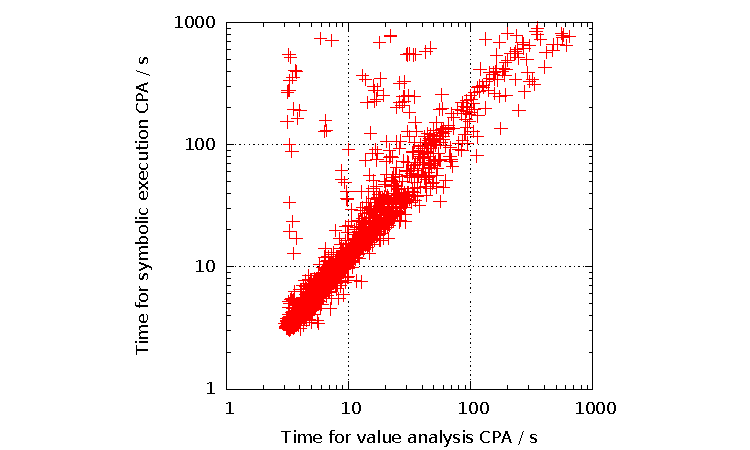
\includegraphics[trim=2cm 0 1cm 0, clip=true, scale=0.9]{evaluation/sp_cputime_VA_symEx}
\caption{Comp. with \valueAnalysisCPA}
\label{fig:valCputime}
\end{subfigure}
\begin{subfigure}[b]{.48\textwidth}
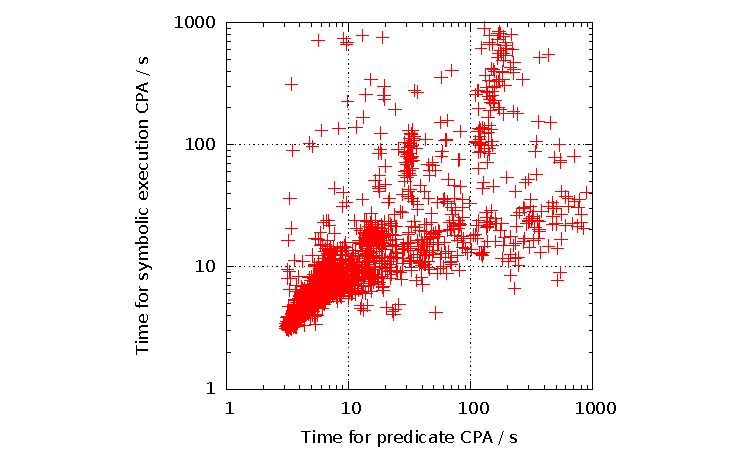
\includegraphics[trim=2cm 0 1cm 0, clip=true, scale=0.9]{evaluation/sp_cputime_pred_symEx}
\caption{Comp. with \predicateCPA}
\label{fig:predCputime}
\end{subfigure}
\caption{Comparison of CPU-time for \valueAnalysisCPA\ and \predicateCPA with \symbolicExecutionCPA\ for tasks each pair computes the same result for}
\end{figure}

\subsection{Predicate CPA}
\begin{table}
\centering
\begin{tabular}{|r|c|c|c|}
\hline
                               & Predicate analysis & Symbolic execution & Overall \\ \hline
correct results                & 2677       & 2476     & 4092 \\ \hline
\resultFalse, correct          & 620        & 476      & 2911 \\ \hline
\resultTrue, correct           & 2057       & 2000     & 1181 \\ \hline
unique \resultFalse, correct   & 262        &  118    & \\ \hline
unique \resultTrue, correct    & 201        & 144         & \\ \hline
\resultFalse, incorrect        & 21         & 94  & \\ \hline
unique \resultFalse, incorrect & 9          & 81         & \\ \hline
\resultTrue, incorrect         & 3          & 1            & \\ \hline
unique \resultTrue, incorrect  & 3          & 1            & \\ \hline
program errors                 & 20          & 3              & \\ \hline % exception because of / 0, parsing error
%timeouts & 3275 & 1927 & \\ \hline
resource errors                & 1317       & 1518      &\\ \hline % includes timeouts + StackOverflowException
\end{tabular}
\caption{Results of benchmarks of the \predicateCPA\ and the \symbolicExecutionCPA, both using CEGAR with sliced prefix selection and the \emph{domain good, short} preference}
\label{tab:predSym}
\end{table}

For comparison to predicate analysis, we used the \predicateCPA\ using bitvector and float theories with its default configuration, using adjustable-block encoding \cite{Beyer2010}.
The sophisticated and evolved \predicateCPA\ is able to outperform symbolic execution in both finding errors and proving programs safe.
It also computes less incorrect results.
Nevertheless, symbolic execution using CEGAR is almost on par with predicate analysis for proving programs safe with only 57~tasks difference.
The \symbolicExecutionCPA\ is able to find errors for 118~programs the \predicateCPA\ can't and prove the safety of programs for 144~programs the \predicateCPA\ can't.
Performance-wise, they differ greatly depending on the task, but with none of them being distinctively better than the other (Fig.~\ref{fig:predCputime}).
In conclusion, the \predicateCPA\ reaches a score of 4572~points in comparison to the \symbolicExecutionCPA's 3906~points.

This shows symbolic execution's potential for software verification, ranked between the \valueAnalysisCPA\ and the \predicateCPA\ in both effectiveness, precision, and performance.

\subsection{Comparison to TRACER}
We tried to compare our symbolic execution approach using CEGAR to TRACER \cite{Jaffar2012a}, a tool for software verification using eager symbolic execution with interpolation.
Unfortunately, TRACER can't handle preprocessed files as they consist in the SV-COMP task sets, by default.
Further investment in making these two tools comparable was not in the scope of this work.
Of the 12~tasks evaluated in \cite{Jaffar2012a}, all but one can be solved by the \symbolicExecutionCPA\ correctly.
TRACER was able to analyze 5~correctly when using strongest-post conditions for interpolation and all of them when using weakest-pre conditions.
Since no information about the evaluation environment is given, it is not reliable to compare the runtime of the analyses.

